
%
\documentclass[%
 reprint,
 amsmath,amssymb,
 aps,
]{revtex4-1}

\usepackage{graphicx}% Include figure files
\usepackage{dcolumn}% Align table columns on decimal point
\usepackage{bm}% bold math


\begin{document}



\title{Comparativa Business Intelligence vs Business Analytics}
\author{Nilson Laura Atencio}
\affiliation{%
 Universidad Privada de Tacna \textbackslash Facultad de Ingenieria \textbackslash Escuela Profesional de Ingenieria de Sistemas
}%

\begin{abstract}
\begin{center}
\textbf{Resumen}
\end{center}

Con el Business Intelligence, a través de una serie de técnicas, se transforman todos los datos de una organización en información, con la cual se podrán identificar posibles indicadores, los cuales serán explotados con objeto de tomar las mejores decisiones. Por ejemplo, listados de ventas o cuadros de control de producción.

El Bussines Analytics, maneja una serie de técnicas (en este caso, utiliza algoritmos predictivos y modelos estadísticos) para transformar los datos en información que tendrá como objeto, predecir posibles resultados (Machines Learnis, Data Minig).



\begin{center}
\textbf{Abstract}
\end{center}
Abstract
With Business Intelligence, through a series of techniques, all the data of an organization is transformed into information, with which you can identify possible indicators, whatever are exploited in order to make the best decisions. For example, sales listings or production control panels. The Bussines Analytics, handles a series of techniques (in this case, uses predictive algorithms and statistical models) to transform the data into information that it will have as its object, to predict possible results (Machines Learnis, Data Minig).


\end{abstract}



\maketitle

%\tableofcontents

\section {Introducción}


Una forma de verlo, es que Inteligencia de negocios (BI) puede considerarse el segmento de tecnológica (modelos multidimensionales, ETLs, self-service, etc.) mientras que BA es más la acción que se da del lado del negocio al tomar decisiones (usando BI cómo parte de los inputs). A manera de analogía, sería como decir que BI es a BA como Data Engineering es a Data Science. ambos conceptos son hermanos y se intersecan. Business Analitycs incorpora Business Intelligence en otras palabras BA es la evolución del BI, tienes análisis descriptivo en BA análisis con predicciones y otros,business analytics él nos va a permitir identificar patrones replantear y hipótesis,pueda ser con ver por ejemplo predecir los costos de generación transmisión distribución y comercialización entonces aquí ya tengo un histórico del costo seguramente con y con los cuales no voy a basar para poder predecir los costos al digamos en el período de tiempo que lo que lo solicite otro escenario puede ser analizar fallos de la infraestructura para en planificación de mantenimientos.
Inteligencia de negocios (BI) es al día de hoy y Analista de Datos (BA)maneja modelos estadísticos para predecir tus indicadores, ejemplo BI te dice cuanto haz vendido y el BA te puede ayudar con tu budget, aunque te debo decir que yo siempre he hecho analytics y no puedes predecir sin analizar el pasado.



%-----------------------------------------------------------------
\section {Marco Teórico}

\subsection{Business Intelligence}

\subsection{Business Analytics}
En términos generales, los sistemas de inteligencia empresarial se utilizan para mantener, optimizar y optimizar las operaciones actuales. El término se refiere a tecnologías, aplicaciones y prácticas para la recopilación, integración, análisis y presentación de información comercial. El propósito de la inteligencia empresarial es apoyar la toma de decisiones empresariales basadas en datos. La inteligencia empresarial a veces se utiliza indistintamente con libros informativos, herramientas de informes y consultas y sistemas de información ejecutiva.
BI mejora y mantiene la eficiencia operativa y ayuda a las empresas a aumentar la productividad organizacional. El software de inteligencia empresarial ofrece muchos beneficios, incluidas potentes capacidades de informes y análisis de datos. Al utilizar los mecanismos de visualización de datos enriquecidos de BI, como paneles en tiempo real, los gerentes pueden generar informes intuitivos y legibles que contienen datos relevantes y procesables.

Entonces, BI ofrece informes y análisis, ¿no son solo dos palabras para lo mismo? Muchas personas, tanto dentro como fuera de la industria del software, utilizan incorrectamente informes y análisis de manera intercambiable, lo que es una de las causas de la confusión detrás de la combinación de BA / BI.
La presentación de informes es "el proceso de organizar datos en resúmenes informativos para monitorear el desempeño de las diferentes áreas de una empresa". Recopila datos y los entrega en un formato digerible.
La analítica es "el proceso de explorar datos e informes para extraer información significativa, que se puede utilizar para comprender mejor y mejorar el rendimiento del negocio". Esta función toma el "qué" de los datos proporcionados por los informes y saca conclusiones e ideas, ofreciendo usuarios un "por qué" y un "cómo". Básicamente, las funciones de informespresentan datos y las características analíticas interpretan los datos. Ambas son características cruciales y generalmente serán ofrecidas por las soluciones BA y BI.

Las visualizaciones de datos tienen un propósito similar al de los informes. Ambas características funcionan como una herramienta para la organización y presentación de datos. Las visualizaciones amplifican las funciones de informes al ofrecer representaciones de datos en un medio fácil de interpretar. Los servicios de decisión reducen el enfoque de la inteligencia empresarial a la información financiera, con muchos sistemas que ofrecen medidas de cumplimiento integradas y detección de fraude.
Las capacidades de integración aseguran que un sistema de inteligencia de negocios pueda funcionar a la perfección con las herramientas actualmente instaladas. Además, las características de integración ayudan a extraer datos de múltiples fuentes, desde bases de datos internas hasta centros Big Data más complejos. Muchas herramientas de BI emplean procesamiento analítico en línea (OLAP) para realizar análisis sofisticados, multidimensionales y detallados
\begin{itemize}
\item Business Intelligence: Conectar a las personas con la información cuándo, dónde y cómo lo necesiten, y colabore para mejorar el rendimiento de negocio.
\item Rendimiento financiero y gestión estratégica: Dirigir la estrategia de gestión hacia los objetivos más rentables mediante información fiable y puntual y la creación de informes transparente y oportuna.
\item Analítica predictiva: Identificar patrones y asociaciones sutiles y desarrollar modelos predictivos para optimizar la toma de decisiones.
\item Gobierno del dato, riesgo y cumplimiento normativo: Obtener un mayor conocimiento en todos los aspectos relacionados con el GRC con una solución integrada cuyos métodos específicos de cumplimiento normativo y de control de riesgos se adaptan a su organización.
\item Aplicaciones analíticas: Proporcionar a los responsables de la línea de negocio el conocimiento accionable con soluciones empaquetadas de análisis y de creación de informes.


	\end{itemize} 

\begin{figure}[htb]
\begin{center}
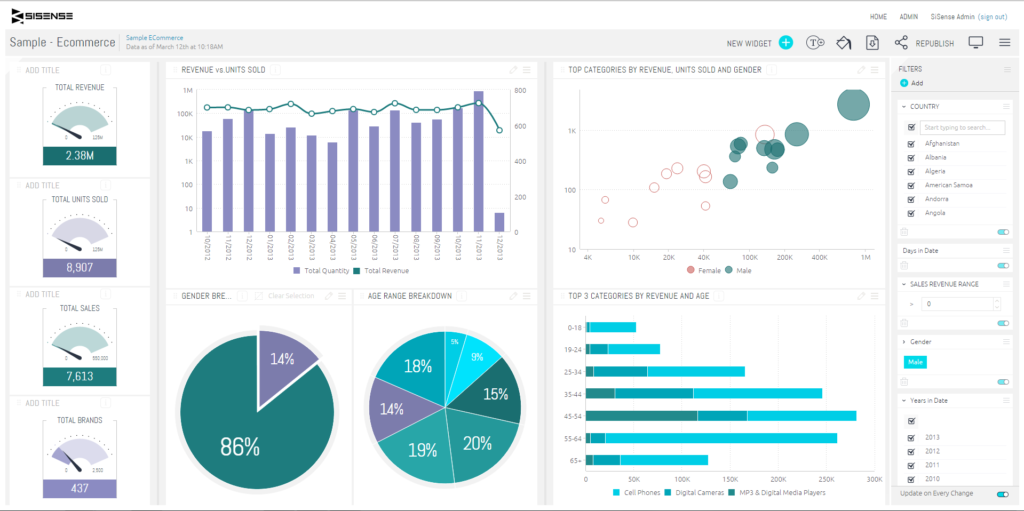
\includegraphics[width=10cm]{./Imagenes/anegocios}
\end{center}
\end{figure}


\subsection{Comparativa}
A continuación, se muestra un cuadro comparativo entre Business Intelligence y Analytics:
\begin{center}
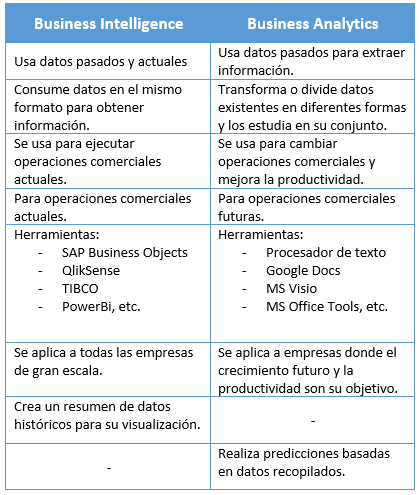
\includegraphics[width=10cm]{./Imagenes/vs1} \cite{hub} \cite{e}
\end{center}

\subsection{Herramientas}
\textbf{Business Intelligence :}
Business Intelligence : Las herramientas de in- teligencia empresarial (BI) son tipos de software de aplicaci´on  que  recopilan  y  procesan  grandes  cantidades de datos no estructurados que proceden de sistemas internos y externos, incluidos libros, publicaciones, documentos,    historias    cl´ınicas,    im´agenes,    archivos, correo electr´onico, v´ıdeos y otros or´ıgenes empresariales. Aunque no son tan flexibles como las herramientas de an´alisis  de  negocios,  las  herramientas  de  BI  ofrecen  un modo  de  acumular  datos  para  encontrar  informaci´on, principalmente mediante consultas. Estas herramientas tambi´en  ayudan  a  preparar  los  datos  para  analizarlos con el fin de crear informes, paneles y visualizaciones de datos.
Ventajas de las herramientas de Business Intelli- gence
- La capacidad de analizar de forma combinada infor- maci´on interna y externa procedente de distintas fuentes y sistemas.
-Una  mayor  profundidad  de  an´alisis  y  una  capacidad ampliada de reporting.
-La   posibilidad   de   remontar   ese   an´alisis   atr´as   en   el tiempo en base a series hist´oricas.
-La  capacidad  de  realizar  proyecciones  y  pron´osticos  de futuro en base a toda esa informaci´on.
 ayudan a preparar los datos para analizarlos con el fin de crear informes, paneles y visualizaciones de datos.\\
\textbf{ Ventajas de las herramientas de Business Intelligence}\\
- La capacidad de analizar de forma combinada información interna y externa procedente de distintas fuentes y sistemas.\\
-Una mayor profundidad de análisis y una capacidad ampliada de reporting.\\
-La posibilidad de remontar ese análisis atrás en el tiempo en base a series históricas.\\
-La capacidad de realizar proyecciones y pronósticos de futuro en base a toda esa información.\\
\begin{itemize}
\item \textbf{IBM Cognos Analytics :}
Es una suite de soluciones de análisis avanzado de información para tomar decisiones: reporting, cuadro de mando, planificación, presupuestación, simulación y análisis cognitivo.
\item \textbf{Microsoft Dynamics :}
Es un sistema de gestión integrada para la empresa, también definido como ERP o Sistema de Planificación de Recursos Empresariales (Enterprise Resource Planning).
\item \textbf{Oracle Business Intelligence :}
Proporciona al usuario un sólido conjunto de informes, consultas ad-hoc, paneles de control y funcionalidad de cuadro de mando. Las soluciones OBIEE son soluciones rentables si la comparamos con una arquitectura orientada a servicios basada en web.
\item \textbf{Style Intelligence:}
Es una plataforma de inteligencia de datos para tableros interactivos, análisis e informes. En su base se encuentra un poderoso motor de mashup de datos que permite una transformación rápida y flexible de datos de fuentes dispares que resuelve los desafíos de administración de datos que otras herramientas de inteligencia empresarial no pueden. Diseñada para una implementación rápida, la aplicación maximiza el autoservicio para una gama de usuarios, desde negocios casuales o navegadores de tipo consumidor hasta usuarios avanzados y científicos de datos.

	\end{itemize} 

\textbf {Business Analytics :}

En el actual mercado, cuando hablamos de Business Intelligence y Business Analytics siempre hay confusión permeando ambas nomenclaturas, principalmente para quienes aún están empezando a entender sus conceptos y cómo aplicarlas. La distinción entre Business Intelligence y Business Analytics es fundamental para su aplicabilidad de forma eficaz en las empresas.
Ambos enfoques están en la punta de un gran cambio y están orientados a proporcionar una visión amplia en la información de negocios. De la misma forma, hay un énfasis creciente en herramientas superiores y softwares más avanzados en la toma de decisiones. Los CEO de empresas a menudo admiten que el business analytics (BA) camina junto con el BI.
A pesar de ser distintas, las dos herramientas están conectadas. Business Intelligence proporciona una manera de acumular datos para encontrar información principalmente a través de preguntas, informes y procesos analíticos en línea. El único problema es que las herramientas de BI estándar no son muy flexibles y la mayoría de las bases de datos no están diseñadas para cambios rápidos.
Por otro lado, el business analytics se aprovecha de datos estadísticos y cuantitativos para modelado explicativo, funcionando como una brújula para organizar la medición de riesgos y prever resultados. El resultado de esta adhesión es una percepción agregada de las informaciones empresariales, creando un nuevo tipo de inteligencia, capaz de optimizar el proceso de toma de decisiones dentro de la organización, capaz de responder a las exigencias inherentes a escenarios cada vez más complejos y competitivos.


\\
\textbf{ Ventajas de las herramientas de Business Analytics}\\
- Te permite tener claridad de los atributos positivos internos de la organización y que están bajo control.\\
- Conocer las fortalezas de los recursos con los que cuentas, las ventajas competititvas de tu organización y fuerza de trabajo.\\
- Te ofrece los componentes internos que añaden valor u ofrecen una ventaja competitiva a tu negocio.\\
\textbf{ Desventajas de las herramientas de Business Analytics}\\
- Se basa en los puntos que están bajo el control de la empresa, limitándose sólo al grado de su propia experiencia, que en ocasiones es limitada.\\
- Al centrarse en los aspectos negativos internos, muchas veces no se toma en cuenta cómo repercute en los servicios o productos que proporciona la empresa. Hay que trabajar todo en conjunto.\\

\begin{itemize}

\item \textbf{ Análisis PESTEL: }
Con esta herramienta de análisis estratégico podremos analizar el entorno en el que queremos crear o establecer nuestra empresa, negocio o proyecto. Nos permite identificar posibles cambios de escenario en nuestro sector o en la región para detectar y aprovechar posibles oportunidades de crecimiento.

\includegraphics[width=8cm]{./Imagenes/img1}
\textbf{ Ventajas}\\
. Muestra en un solo informe el entorno de nuestra organización\\
. Descubrimiento de oportunidades y amenazas\\
. Nos ayuda a planificar\\
. Herramienta sencilla de utilizar\\
\textbf{ Desventajas}\\
- Posibilidad de pasar por alto información relevante si no se realiza de manera exhaustiva, hay que dotarlo de un enfoque profundo\\
- Necesidad de actualización periódica, especialmente en sociedades en rápido desarrollo\\
- La información necesaria no siempre es fácil de conseguir (ni barata)\\
- Las estrategias pueden no ser las más convenientes si no se realizan de manera adecuada\\
- Dificultad para establecer modelos sobre lo que va a pasar en el futuro

\item \textbf{ Análisis FODA: }
El análisis FODA es una herramienta de planificación estratégica, diseñada para realizar una análisis interno (Fortalezas y Debilidades) y externo (Oportunidades y Amenazas) en la empresa. Desde este punto de vista la palabra FODA es una sigla creada a partir de cada letra inicial de los términos mencionados anteriormente.
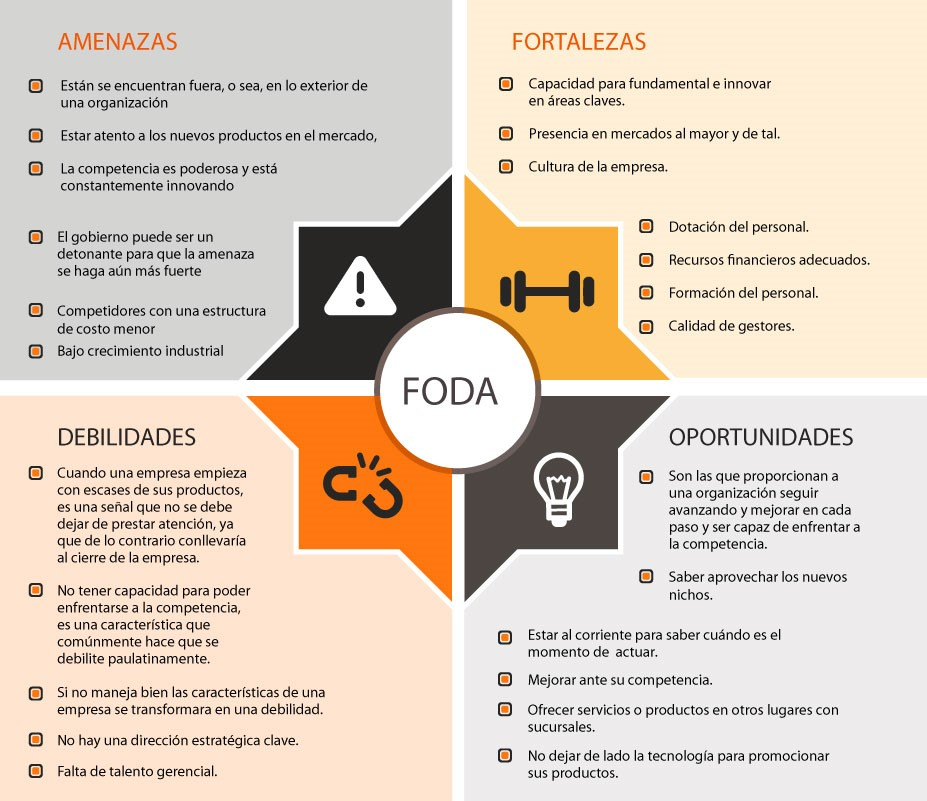
\includegraphics[width=6cm]{./Imagenes/img2}\\
\textbf{ Ventajas}\\
. Muestra en un solo informe el entorno de nuestra organización\\
. Descubrimiento de oportunidades y amenazas\\
. Nos ayuda a planificar\\
. Herramienta sencilla de utilizar\\
\textbf{ Desventajas}\\
. Posibilidad de pasar por alto información relevante si no se realiza de manera exhaustiva, hay que dotarlo de un enfoque profundo\\
. Necesidad de actualización periódica, especialmente en sociedades en rápido desarrollo\\
. La información necesaria no siempre es fácil de conseguir (ni barata)\\
. Las estrategias pueden no ser las más convenientes si no se realizan de manera adecuada\\
. Dificultad para establecer modelos sobre lo que va a pasar en el futuro\\

\item \textbf{ Modelo de las 7 S: }
Las fortaleza de las 7S  es que es una herramienta de diagnostico para entender por qué las organizaciones son ineficaces. Una vez analizados los puntos débiles y realizados cambios, se conduce a un cambio organizacional, implicando al total de la compañía que puede hacer mejorar significativamente su forma de funcionar y sus resultados.
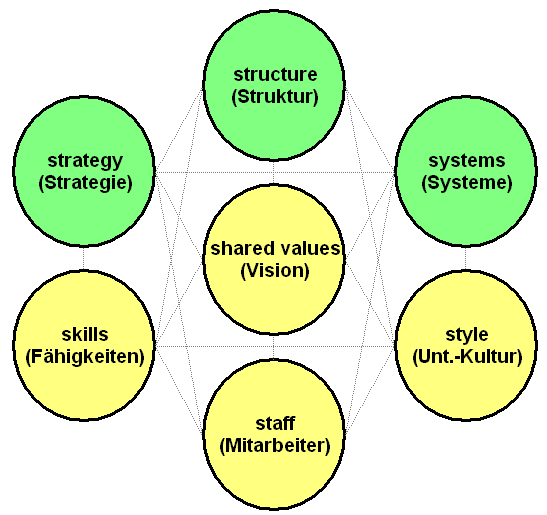
\includegraphics[width=8cm]{./Imagenes/img3}

	\end{itemize} 

%-----------------------------------------------------------------
\section{Análisis}


%-----------------------------------------------------------------
\section{Conclusiones}
\begin{itemize}
\item En forma exclusiva, la inteligencia empresarial y el análisis de negocios forman los componentes esenciales requeridos por una empresa para administrar su información de manera efectiva.
\\
\item 
En conclusion, los sistemas de inteligencia empresarial se utilizan para mantener, optimizar y optimizar las operaciones actuales. El término se refiere a tecnologías, aplicaciones y prácticas para la recopilación, integración, análisis y presentación de información comercial. El propósito de la inteligencia empresarial es apoyar la toma de decisiones empresariales basadas en datos

\\
\item En un medio globalizado y audaz como el del mundo empresarial, podemos ver que el entorno en el que la inmensa mayoría de las empresas tiene soportados los procesos de negocio con diferentes sistemas de información y estrategias, los ubica en un mercado tan competitivo como el actual, Hoy se ha convertido en un problema, por lo que la Inteligencia de Negocios se erige como una pieza clave para ser proactivo a la hora de tomar mejores decisiones y de conseguir mejor control de negocio y ventajas que nos diferencien de la competencia.
\\
\item la gran mayoría de empresas no utilizan sistemas de inteligencia empresarial para gestionar sus negocios. Sin embargo, entienden el concpeto y saben que son herramientas muy enriquecedoras para la gestión actual.
\end{itemize} 



% Bibliografia.
%-----------------------------------------------------------------

\bibliographystyle{plain}
\bibliography{Bibliografia}

\end{document}

